\documentclass[nobib]{tufte-handout}
%\geometry{showframe} % for debugging purposes -- displays the margins
\usepackage{amsmath}

% Set up the images/graphics package
\usepackage{graphicx}
\setkeys{Gin}{width=\linewidth,totalheight=\textheight,keepaspectratio}
\graphicspath{{graphics/}}

\title[Psychological Acculturation - Narrative]{Psychological Acculturation: \\
Adjusted Narrative Structure with Notes}
\author[Kreienkamp et al.]{}
\date{March 28, 2021}  % if the \date{} command is left out, the current date will be used

% The following package makes prettier tables.  We're all about the bling!
\usepackage{booktabs}

% The units package provides nice, non-stacked fractions and better spacing for units.
\usepackage{units}

% The fancyvrb package lets us customize the formatting of verbatim environments.  We use a slightly smaller font.
\usepackage{fancyvrb}
\fvset{fontsize=\normalsize}

% Small sections of multiple columns
\usepackage{multicol}

% Provides paragraphs of dummy text
\usepackage{lipsum}

% strike out text
\usepackage[normalem]{ulem}

% APA citations
\bibliographystyle{plain}
\usepackage[style=apa, sortcites=true, sorting=nyt, backend=biber, natbib=true, uniquename=false, uniquelist=false, useprefix=true]{biblatex}
% add reference library file
\addbibresource{references.bib}

% These commands are used to pretty-print LaTeX commands
\newcommand{\doccmd}[1]{\texttt{\textbackslash#1}}% command name -- adds backslash automatically
\newcommand{\docopt}[1]{\ensuremath{\langle}\textrm{\textit{#1}}\ensuremath{\rangle}}% optional command argument
\newcommand{\docarg}[1]{\textrm{\textit{#1}}}% (required) command argument
\newenvironment{docspec}{\begin{quote}\noindent}{\end{quote}}% command specification environment
\newcommand{\docenv}[1]{\textsf{#1}}% environment name
\newcommand{\docpkg}[1]{\texttt{#1}}% package name
\newcommand{\doccls}[1]{\texttt{#1}}% document class name
\newcommand{\docclsopt}[1]{\texttt{#1}}% document class option name

% make question with red triangle
\newcommand\Question[1][2ex]{%
  \renewcommand\stacktype{L}%
  \scaleto{\stackon[1.3pt]{\color{red}$\triangle$}{\tiny\bfseries ?}}{#1}}%
  
% add definition sections
\newtheorem{definition}{Definition}

% add quote section
\usepackage{csquotes}

% framed box section
\usepackage{framed}
\emergencystretch=1em

\begin{document}

\maketitle % this prints the handout title, author, and date

\begin{abstract}
\noindent\marginnote{Abstract: 117 words}One of the key challenges to researching psychological acculturation is an immense heterogeneity in theories and measures. These inconsistencies make it difficult to compare past literature on acculturation, hinder straight-forward measurement selections, and hampers the development of an overarching framework. To structure our understanding of the migration process, we propose to utilize the four basic elements of human experiences (motivations, emotions, thoughts, and behaviors) as a conceptual framework. We use this framework to build a theory-driven literature synthesis and find that the past methodological and empirical literature as well as theoretical models have understudied the more internal aspects of acculturation (motivations and emotions) and have often fallen short of capturing all four aspects of the migration experience.
\end{abstract}

%\printclassoptions

\newthought{Relevance}\marginnote{Maybe replace with refugee crisis example.}
The question of how people change when they get into continuous first-hand contact with other cultures is probably as old as the history of human migration and remains an important issue for many societies around the world. 
Almost 4,000 years ago Ipuwer of Egypt wrote "those who were once Egyptians [have become] aliens" (\citeauthor{Ipuwer2003}, ca. 1250 B.C.E./2003, Admonitions of Ipuwer 4:1) because of their contact with foreigners. Nearly 2,000 years later Plato similarly bemoaned the "blending of characters" (\citeauthor{Plato1926}, ca. 384 B.C.E./1926, Laws 12:949e ff.) when the good people of Athens got into contact with other cultures. Another 2,000 years later, over the past 80 years, researchers of the psychological sciences have proposed hundreds of models and measurements for this phenomenon of "psychological acculturation" \citep[][]{Rudmin2003a}. Yet, despite enormous theoretical and applied advances, it remains unclear what exactly we mean when we talk about psychological acculturation. A conceptual framework allowing for a synthesis of the past literature on psychological acculturation is still missing \citep{Birman2014c}.

\newthought{Problem}\marginnote{Still need to be toned down. Kai: simply point out the different fields that have focused on the topic.}
This absence of a conceptual framework presents fundamental challenges to researchers, practitioners, and policy-makers in the field. The scattered conceptualization causes issues in the synthesis of past literature and the development of new theories and measurements.
Looking back at past theories and measures, the diversities of included or excluded constructs makes it virtually impossible to compare different effects and outcomes, which makes it difficult to integrate them without a framework that comprehensively organizes the different aspects \citep{Taft1981}\footnote{\textit{"The conceptualization and methods are so variant that it is almost impossible to integrate them, whether intuitively or by some objective procedure such as a formal meta-analysis."} \citep[p. 343]{Taft1981}.}.
Looking forward, it in turn remains difficult to select past elements and develop new theories and measurements. A conceptual framework would be necessary to make informed and transparent choices on which aspects are (ir)relevant to a given research question and how they relate to one another.
Given these challenges, some have even suggested that psychological acculturation should not be measured until common terminologies and frameworks are available \citep{Escobar2000}.

\newthought{Aim} The aim of this paper is, therefore, to offer a descriptive conceptual framework to analyze, measure, and understand the concept of psychological acculturation. Such a framework has a different objective than previous efforts to catalogue literature on cultural adaptation \citep[e.g.,][]{Castels2003}, build multidimensional measures of integration \citep[e.g.,][]{Harder2018}, normative frameworks \citep[e.g.,][]{Ager2008a}, or theories of acculturation \citep[e.g.,][]{Berry2005}. Rather than offering a new measurement, definition, or theory, we aim to build a framework to assess and compare any of these conceptual elements. 
Building on past reviews, we propose to do so by using the basic elements of human experiences and motivation to structure the concept of cultural adaptation.
Once we have introduced our conceptual framework, we will systematically review the past methodological, applied empirical, and theoretical literature on acculturation to apply the framework. This should also allow us to synthesise a status quo of the scattered literature and identification of gaps within it.

\section{Definition and Focus}\label{sec:definition}The most widely reported definition of 'acculturation', as it is understood within the psychological tradition, is probably the definition by the Social Science Research Council \citep[][p. 149]{Redfield1936}:
\begin{framed}
    \begin{definition}[Acculturation]
        Acculturation comprehends those phenomena which result when groups of individuals having different cultures come into continuous first-hand contact, with subsequent changes in the original culture patterns of either or both groups.
    \end{definition}  
\end{framed}
Following this definition, acculturation is any observable event (i.e., phenomenon) or change that is due to a contact with a new culture. Notably, the terms of “phenomena” and “changes” remain decidedly vague and define acculturation as both a process and an outcome at the same time. Moreover, the phrase "groups of individuals" suggests that acculturation occurs as two related, yet separate, processes of cultural and psychological acculturation \citep[also see,][]{Sam2006b, Berry2005}.

In this review we will focus on the individual level and assess aspects of 'psychological acculturation', as that is the focus of psychological research. For this more micro level concept many have used the definition proposed by \citet[][p. 14]{Sam2006b}, based on a research paper by \citet{Graves1967}: 
\begin{framed}
    \begin{definition}[Psychological Acculturation]
        “Psychological acculturation” refers to the changes an individual experiences as a result of being in contact with other cultures, or participating in the acculturation that one’s cultural or ethnic group is undergoing (Graves, 1967).
    \end{definition}
\end{framed}
Here the main focus of the definition lies on the "individual experiences", which is in direct concordance with our proposal to use the elementary aspects of the human experience to structure the concept of psychological acculturation.

Another important focus distinction commonly found within the psychological literature is the differentiation between majority and minority culture members. While psychological acculturation can apply to any inter-cultural contact \citep[including, for example, the contact between indigenous people and colonial settlers, e.g.,][]{Berry1974}, a majority of theories and studies have focused on cross-national immigrants. And while the framework we propose is applicable to psychological acculturation in its wider sense, its development and our focus in the following sections will lay mainly with the experience of minority immigrants.

\section{Conceptual Framework} 

To build a framework that would comprehensively structure the concept of psychological acculturation across a wide range of contexts, we propose to utilize the structural elements of human experiences and motivation. This framework was developed based on collaborations with resettlement organizations and migrant citizens as well as based past reviews and theoretical developments within the field. We will introduce each of these sources and the development in short before we discuss the structural elements in more detail and apply the framework to the systematic literature review.

\subsection{Focus Group Discussion}
In a first step we reached out to societal stakeholders of the acculturation process to gather information on key adaptation aspects in the lived realities out in the field. These experience reports formed the earliest foundation of our framework aspects. The focus group consisted of migrants, refugees, teachers, language- and integration coaches, volunteers and staff of a regional refugee resettlement agency as well as a representative of the local government. The 12 carefully selected and invited participants joined a 120 minutes round-table focus group discussion on the concept of acculturation. With informed consent by the participants, the discussion was audio recorded, transcribed, and later coded in three coding cycles of (1) initial In Vivo coding using the participants own words, (2) open coding inductively identifying common topics and elements, as well as (3) a content analysis using focused coding to summarize the overarching themes, which included the experience elements discussed here.

%\newthought{One Paragraph Version}\marginnote{This seems a bit too short to me.}\\
%During the analysis of the focus group discussion a range of experience elements emerged as key elements around which the discussion evolved. While individual differences in contexts, personality, and situations were often highlighted and discussed, there was a broad consensus within the group that the individual experience of the newcomer should function as a starting point for understanding psychological acculturation. Accordingly, during the content analysis behaviors, emotional experiences, thought processes, and needs or wishes were the most elemental themes that structured the discussion content. Over the two hour period, the conversation between the participants notably evolved from public and visible aspects of the acculturation experience (particularly, language learning and social contact behaviors) to more internal aspects of the experience (including, identity developments, feeling at home, and wishes to be accepted). We discuss a number of examples with participant quotes within the supplementary materials (see, SI X).

\paragraph{Behavior} As behaviors are often a particularly visible aspect of cultural interaction processes, the discussants elaborately discussed the social-behavioral acculturation aspects and expected behaviors in the new environment. The group particularly highlighted language learning and social contacts as examples of prominent behavioral acculturation aspects. Importantly, these behaviors were not only highlighted as a process towards acculturation but as an integral part of acculturation itself. For example, to have interactions outside the home was described as an important part of connecting to the culture and to being seen as an active member of society. Importantly, the group also discussed that many (interactive) behaviors are reciprocal and reactive in nature, depending on the collaboration with majority group members.
\begin{displayquote}
    Maria:\\
    {[...]} \textit{while, of course, you integrate best when you go to work.}
    
    Moderator:\\
    \textit{Why is that exactly?}
    
    Maria:\\
    {[...]} \textit{Because there you have daily contacts with locals.}
\end{displayquote}

\paragraph{Cognition} The round table discussion also highlighted the newcomer’s cognitive development as a key process of psychological acculturation. One aspect prominent during the discussions was that 'how we think about ourselves and the world' is often integral for navigating a new environment --- including, for example, language, social- and communication norms. A second major topic discussed was the role of identity development. The newcomers pointed to both a break in identity (the struggle of defining oneself in the new environment) as well as the struggle of dealing with a singular (migrant or refugee) identity label and the process of developing a more complex identity narrative towards others. Another key discussion point was that many behaviors are partly in service of cognitive acculturation. Participants, for example, highlighted that through interactions with majority group members migrants can learn about the social system, values, and social rules.
\begin{displayquote}
    Yahya:\\
    {[...]} \textit{Once I started my education, I felt part of society. That was actually a really big difference. That I have friends at my school. That is when ... I felt that I was a part of society. And that is a very big difference to before. That was not the case when I was learning Dutch at the university, at the language school, or at other places before. Only later when I was at school, ... I feel: Okay, now I feel I am really in the Netherlands.}
    
    Joop:\\
    \textit{Why did you not have that at the language school?}
    
    Yahya:\\
    \textit{Because I was only a refugee.}
\end{displayquote}

\paragraph{Affect} When the discussions turned to affective components of the acculturation process, the main and underlying sentiment was that the emotional aspects of acculturation foreground the importance of the subjective experience as acculturation. Instead of focusing on purely behavioral outcome conceptualizations (e.g., housing, job, education), the group highlighted the importance of considering the affective acculturation experience (e.g., feeling at home, feeling accepted). As an example, when asked why having a job is important to acculturation, newcomers and supporters pointed to a feeling of usefulness and being part of society. Similarly, the group pointed out that learning the local language was not only important to contact and communication but to feeling welcomed and judging the extend of acceptance. 
\begin{displayquote}
    Fariq:\\
    {[...]} \textit{But for me the language is very very difficult. And then you think people are not open. And you don't understand because your language isn't that good. And then you maybe don't feel welcomed when I have questions or want to approach them. But when you learn the language and then get into contact with people, ... then you know whether you are accepted or not.}
\end{displayquote}

\paragraph{Desire} The motivation aspect of acculturation was likely discussed in the most interesting way during the focus group discussion. The (lack of) motivation to interact with the new culture and its members was one key discussion point but motives for actions and psychological needs of the migrants were also discussed as more impalpable properties of other acculturation aspects (e.g., the need for acceptance during interactions). Yet, importantly the motivational aspect also highlighted the functional essence of individual acculturation. The needs for interactions, to be understood, for purpose, and for identity continuity were discussed as not only expected by the host majority but as intrinsic and fundamental to the health and functioning of the newcomers as part of the acculturation process.

\paragraph{Complex Experience Process} It remains important to point out that these themes emerged as part of the focus coding but were not discussed in isolation from one another. The group, for example, pointed out that most of the cognitive and affective acculturation aspects are often facilitated through (structured) social behavioral activities such as school, work, sports, music, and associations. Similarly, the feelings of becoming part of society (including descriptions of feeling useful, self-esteem, and purpose) were related to behavioral adaptation (contact, and work), and cognitive adaptation (developing a complex identity not just refugee identity). Moreover, the group also highlighted during their discussions, that in practice acculturation was mostly a developmental or temporal process rather than a static end goal. While the group did discuss possible comparisons of how one person might be more acculturated than another, an overwhelming majority of the discussion centered around the acculturation process and aspects that are elementary to any migration experience. In sum, the voices of experts in the field and of those actively going through the migration and inter-cultural contact process highlighted the importance of focusing on the individual experience in order to comprehensively understand the elements of the concept.

\subsection{Past Literature}
The focus group discussion, thus, inspired this undertaking and laid the groundwork for the development of an experience framework of psychological acculturation. Yet, at the same time, the framework also grew out of a strong theoretical tradition in the field and arguably brings together many of the past advances in capturing psychological acculturation. The literature on psychological acculturation has grown exponentially over past decades \citet{Rudmin2003a} and several reviews \citep[e.g.,][]{DeLeersnyder2017, Matsudaira2006, Celenk2011}, conceptual reflection papers \citep[e.g.,][]{Ward2012, Berry1997b}, and even a handbook have been published \citep{Sam2006a}. 

In recent years, there seems to form a theory-level agreement that the psychological acculturation process can be separated by its time-scale. The more short-term process of change is usually referred to as the acculturation orientation \citep[e.g.,][]{Ward2001, Berry2003} and is commonly based on Berry and colleagues (\citeyear{Berry1997b, Berry2003}) acculturation attitudes. This orientation describes a two-dimensional process of changes in peoples' preferences of their heritage culture and the new culture --- in terms of attitudes, attachments, goals, identifications, as well as choice and use of cultural elements, such as language, foods, or dresses.
The longer-term changes as part of the acculturation concept are commonly referred to as psychological and socio-cultural adaptation \citep{Searle1990, Ward2001, Berry2003} and can include aspects such as satisfaction and well-being, as well as cultural skills and performance. Over the broader acculturation process, there are thus a wide range of aspects that change within an individual.

Adding to the conceptual difficulties is the case that in empirical practice orientation and adaptation distinctions are less commonly observed (for exceptions see \citealp{ICSEYteam2006, Berry2006b, TeLindert2008a}). Instead, researchers more commonly focus on acculturation in terms of different 'acculturation aspects' \citep{Arends-Toth2006a}, which might include any of the orientation, identity, or adaptation elements. In sum, it thus remains unclear what aspects the concept exactly entails, how these aspects are organized, and measurements are inconsistent across studies and interventions.

In response to the immense diversity of perspectives within the acculturation literature, Ward and colleagues \citep{Ward2001, Masgoret2006, Ward2019} proposed that the theoretical perspectives commonly found within the literature can be separated into three main traditions\footnote{\citet{Ward2001} mentions six bodies of literature but does not specify further.}. Ward and colleagues have labeled these traditions affect, behavior, and cognition (forming the ABCs of acculturation). Within the affective tradition Ward situates the stress and coping literature., behavioral traditions are the cultural learning theories, and social identification theories form the cognitive theories.

\citet{Sam2006b} and others have noted that such a perspective might be useful in structuring the core components of psychological acculturation. We agree and see a broader potential to apply this to the concept of psychological acculturation in general, proposing an expanded ABCD structure, which includes desires (i.e., motivational literature). 

\newthought{Experience} Beyond the intuitive appeal of an ABC(D) separation we belief that such a framework also has the potential to offer a theory-driven literature synthesis. A growing body of literature suggests that human experiences can be understood as a set of needs, emotions, cognitions, and behaviors \citep[sometimes referred to as the ABCs or ABCDs of psychology: affect, behavior, cognition, desire; e.g.,][]{Cottam2010, Hogg2005, Jhangiani2014}. \footnote{It should also be noted that ABC(D) frameworks have been used effectively to structure theories and models across a wide variety of fields --- including research on attitudes \citep{Breckler1984} and ambivalence \citep{VanHarreveld2015}, self-regulation \citep{Ben-Eliyahu2015}, the big five personality traits \citep{Wilt2016}, suicidality \citep{Harris2015} and in clinical interventions \citep{Eifert1989}, and even the review of acculturation literature \citep{Ward2001, Ward2019}. Interestingly, the affect, behavior, and cognition structure has even found application in the development of human-like machines \citep{Guo2020}.} Following the premise that any human experience can be perceived within these four basic elements, we belief that the an ABCD framework of psychological acculturation would not only summarize theoretical traditions within the acculturation literature, but could offer a comprehensive and theory-driven framework to structure and analyze the concept of psychological acculturation.

\newthought{Examples} Psychological acculturation in this framework might, for example, be understood or measured in terms of behavioral acculturation, such as language use, or voting; cognitive acculturation, such as ethnic identification, or cultural values endorsement; affective acculturation, such as feeling at home, or loneliness; motivational acculturation, such as the satisfaction of competence or independence needs; or as a complex combination of any or all of these aspects (also see Table \ref{tab:Examples}1 for a range of examples). 

\begin{table}[hbt!]
\caption{Examples for Acculturation Aspect Measures (To be combined with Table 3)}
\label{tab:ExamplesTab} 
\begin{tabular}{@{}llll@{}}
\toprule
Affect              & Behavior                                     & Cognition                          & Desire                \\ \midrule
Lonely              & Language   use                               & Ethnic   identification            & Competence            \\
Feeling at home     & Civic   Participation (voting, ...)          & Cultural   values                  & Independence          \\
Satisfied with life & Performance   (work, ...)                    & Acculturation   orientation        & Self-coherence        \\
Proud               & Media   consumption                          & Preferences   (food, friends, ...) & Belonging             \\
Comfortable         & Education                                    & Knowledge                          & Achievement           \\
Enjoy               & Peer   contacts                              & Importance   ratings               & Justice               \\
At ease             & Food   consumption                           & Inner   thought language           & Growth                \\
Well-being          & Cultural   habits (holidays ...) & Perceived   obligations            & Respect               \\
Worry               & Delinquance                                  & Beliefs                            & Acceptance            \\
Trust               & Marriage                                     & Stereotypes                        & Identity   continuity \\
...                 & ...                                          & ...                                & ...                   \\ \bottomrule
\end{tabular}
\end{table}

\subsection{Framework Elements}

In the next sections we will look at past literature on each of the aspects in more detail to discuss how the experience aspects relate to the concept of psychological acculturation. 

\paragraph{Affect}entails the human capacity to feel \citep[including emotions and moods;][]{FeldmanBarrett2007}. These affective experiences are profoundly differ between cultures \citep[e.g.,][]{Holodynski2012, Boiger2018} and inversely emotions are an integral part of cultures and their narratives \citep{Ahmed2014, Kitayama1994, Smith2016c, Sundararajan2015}. Their experience and expression is, thus, often a key aspect when two cultures come into contact \citep[e.g.,][]{Iyer2008, Stephan1992}. Moreover, more broadly, emotions have long been a gauge of adaptation to social change and major life events \citep[e.g.,][]{Smith1990, Pacella2017}. Phenomena such as culture shock \citep{Ward2001a} and homesickness \citep{VanTilburg1996} are common examples of how social change can have an emotional impact on well-being and might function as an indicator of adaptation. Previous literature has, thus, established a deep connection between affect and cultures, cultural contacts, as well as adaptation.

From these findings it is not surprising that affect and emotion have also been discussed within the psychological acculturation literature. \citet{Ward2001} in her review of the acculturation traditions, describes the stress and coping literature --- especially Berry's concept of acculturation stress \citep{Berry1997b} --- as the affect component of acculturation. In this tradition, the main constructs that constitute the affective dimension are the psychological and emotional well-being as part of the psychological adaptation process \citep[including, for example life satisfaction and depression][]{Ward2019}. However, beyond the theoretical stress literature tradition, there are also more immediate models and measurements of emotional acculturation. There is, for example, a relatively young tradition of 'emotional acculturation' as a distinct concept in which acculturation is understood as the similarity in emotional patterns \citep[see][for a review]{DeLeersnyder2017}. But also individual emotions, such as 'feeling accepted' \citep{Jasini2018}, or 'pride' \citep{Suinn1995} have received attentions as discrete aspects of acculturation. 

\paragraph{Behaviors}--- that is actions and mannerisms --- are often learned (i.e., extra-somatic or extra-genetic) and especially social behaviors are often culturally transmitted \citep{Legare2019, Whiting1980}. Cultural differences are, thus, often most visible in behavioral differences, including language use, dress- and food preferences, rituals and habits, as well as behavioral norms more generally \citep[e.g., social norms, as well as formal rules and laws; e.g.,][]{Hofstede2001}. And, inversely, behaviors are also an important aspect of what we consider culture \citep[e.g.,][]{Varnum2017}. One prominent recognition of this relationship between culture and behavior, has been the protection of indigenous cultural practices as a manifestation of their culture \citep[Art. 11]{UnitedNations2007}. Behaviors and their norms are, thus, a key component when cultures get into contact \citep[also see][]{Maxwell2017, Sam2010}. And also in a broader notion, behavioral changes have long been considered within the adaptation and well-being literature \citep[e.g.,][]{Luhmann2012}. In sum, behaviors lay at the very foundation of many cultural contacts and can be essential in forming an adaptive relationship with one's environment.

Given the overt nature of behaviors and their interconnectedness with culture, behaviors have also been a prominent aspect of the acculturation literature. Ward and colleagues \citeyear{Ward2019} in their review have identified cultural learning theories as one key literature tradition that has focused on behavioral aspects of acculturation. They relate these learning theories to the acquisition of effective skills and competences as the behavioral operationalizations \citep[including, verbal and non-verbal communication skills][]{Ward2001}. Other examples of behavioral conceptualizations of acculturation (not mentioned by Ward and colleagues), include civic participation \citep[e.g., voting;][]{Lessard-Phillips2020}, inter-ethnic marriage \citep[e.g.,][]{Song2009}, and media consumption \citep[e.g.,][]{Shoemaker1985}. 

\paragraph{Cognition}aspects commonly entail the thinking processes of the human experience and thus include cultural knowledge, values, identities, beliefs, and attitudes, which are likely the most widely discussed aspects of non-material culture \citep[e.g.,][]{DiMaggio1997}. Yet at the same time cognitions are also substantially influenced by culture \citep[e.g.,][]{Gelfand2011, Nisbett2002}. As such, cognitions and their affordances often structure inter-cultural contacts \citep[e.g., values;][]{Ramstead2016} and contact perceptions \citep[e.g., out-group attitudes;][]{Stephan2000a}. Moreover, processes such as meaning making, self-image restoration, and dissonance reduction have established cognitive adaptation as a vital element in well-being and adaptation processes \citep[e.g.,][]{Czajkowska2017}. In sum, cognitions are a prominent aspect of the human experience intimately intertwined with conceptions and influences of culture. Cognitions also structure and gauge cultural contacts and are a key process of human adaptation.

Given the pertinent connection between culture and cognitive processes, it might come as little surprise that cognitions have also played a major role in the acculturation literature. \citet{Ward2001} have identified literature traditions on ethnic identity and group perceptions within the field. Within this cognitive tradition, Ward and colleagues particularly focus on Berry's \citeyear{Berry1997b} acculturation attitudes \citep{Ward2019}. Beyond the cultural attitudes tradition, the acculturation literature has recently also focused on several other cognitive conceptualizations of psychological acculturation, including cultural values \citep[e.g.,][]{Marin2003} and stereotypes \citep[e.g.,][]{Stanciu2018}. 

\paragraph{Desire} here encompasses the motivational forces of the human experience and there is substantial evidence that many of the psychological wants and needs are culture specific \citep[e.g.,][]{McInerney2016, Morling2017}. Yet, inversely the cultures themselves in part consist of motivational ideals \citep[or oughts; e.g., see][]{Markus1991}. Given this link to culture it is not surprising that psychological needs have recently also been highlighted as a key element in inter-group and inter-cultural relations \citep{Dovidio2017, Kitayama2007, Hassler2021, Shnabel2008a}. But also more broadly, needs have long been linked to different well-being regulations \citep[e.g.,][]{Steverink2006} and recently first evidence has emerged showing how motivations might fundamentally drive adaptation processes \citep{Dignath2020}. 
In sum, motivation has a deep connection to culture, cultural contacts, and psychological adaptation.

Yet, despite these connections, motivation is seldom discussed as a distinct aspect of the psychological acculturation concept. Few of the past reviews have examined its role within the literature or the concept \citep[including, ][]{Ward2001a, Ward2019}. However, in recent years needs and wants have been discussed more frequently as a conceptual aspect of psychological acculturation --- with more researchers looking at migration driven by reason for migration \citep{Sandu2018}, as well as the motivations of acculturation orientation s\citep{Recker2017a}, acculturation behavior \citep{Reece2000}, and psychological adaptation \citep{Safdar2003}. 

\paragraph{Process}
%% Dynamic process rather than static end-product: 
% Experience can answer this call because it can only be understood based on past experiences
A final, fundamental factor we would like to address in the experience framework is the understanding of psychological acculturation as a dynamic process rather than a static end-product. That psychological acculturation is a developmental process, and that ``acculturation occurs when two independent cultural groups come into \textit{continuous first-hand contact over an extended period of time}'' \citep[][186]{Berry1989} seem to be a generally accepted assumption within the field\footnote{also see '\nameref{sec:definition}' section}. Yet, some reviews have pointed out that applied studies have actually considered the theoretical implications of migration as a process and even fewer have methodologically followed the trajectories of migrants over time \citep[e.g.,][]{Brown2011, Ward2019}. We believe that the experience framework of psychological acculturation, as it is presented here, is ideally suited to deal with this conceptualization as a developmental process. Philosophers of the phenomenological tradition have long highlighted that subjective experience can only be understood within the history of past experiences \citep[e.g.,][]{Heidegger1867}. 

\paragraph{Experience elements and lived experience}
While we have introduced the four experience aspects as distinct elements it is important to note that both in theory and in practice affect, behavior, cognition, and desire are not experienced as distinct entities. As an example, most emotions have a cognitive component just as most cognitions have an emotional value. Similarly, motivation is commonly conceives as having both emotional (e.g., desire) and cognitive (e.g., goals) aspects, both of which are often directed towards behaviors (i.e., conation). Muddying the waters further is the difficulty that many operationalizations (and empirical measures) of psychological acculturation are complex concepts in themselves. Concepts such as satisfaction or distress, which are common measures of acculturation, famously include emotional and cognitive components. 

Yet, despite the interdependence of aspects and the complexity in the lived experience, the four elements can consistently be identified within experiences and concepts --- they remain qualitatively different aspects of the experience. And as such, they offer a pragmatic lens to structure the psychological acculturation concept \citep{Kuhn1962}. Differentiating the four (needing, feeling, thinking, doing) qualities of an experience in the what we consider psychological acculturation to be, allows us to structure our discussions of past, current, and future theories and measures of psychological acculturation.

\newthought{Features}\footnote{Not an actual heading I think} 
Now that we have introduced the individual experience elements in detail, we would like to speak to the qualities of such a framework more broadly. We belief that utilizing the elements of the human experience to structure the concept of psychological acculturation offers a set of valuable features, which address past conceptual issues. 

Firstly, the experience approach is based on basic human faculties, that is generally speaking every healthy person has the capacity for emotions, thoughts, needs, and behaviors. Focusing on fundamental faculties relevant to any conscious person makes the framework widely applicable across cultural contexts. ABCD frameworks have, for example, been found across cultures \citep[e.g.,][]{Bhawuk2011} and likely structure human forebrain functioning \citep{Swanson2020}\footnote{Probably move to discussion: It is important to note that while anyone will have motives, emotions, thoughts, and behaviors, what one needs (e.g., belongingness or independence), feels (e.g., sadness or happiness), thinks (e.g., identification or disinterest), or does (e.g., studying or working) is highly ideographic. It is this ideographic content that makes the framework relevant to such a broad range of migration contexts. Yet it is the content-free structure --- the presence or absence of the basic elements in conceptualizations of acculturation --- that is transferable across contexts and studies, enabling comparisons and broader conceptual discussion. It should also be noted that in our opinion such a framework does not stand in conflict with cultural or indigenous psychological concerns of an absolutist, or deterministic psychology \citep[e.g.,][]{Kim2006a}. In fact, cultural psychologists, together with many decolonial researchers, have long argued that the individual embedded and lived experience should gain a more central role in our theoretical developments \citep[e.g., ontological turn;][]{Pedersen2020}}.

Secondly, because affect, behavior, cognition, and desire broadly capture the human experience, the experience framework comprehensively captures the psychological element of acculturation. The framework, thus, captures a broad and complex phenomenon while still offering a clear and theory-driven structure of the concept and its applications. 
As such it focuses on how individuals perceive the acculturation process. This also means that non-psychological aspects such as biological, cultural, or societal changes are not captured directly but only to the extent to which they impact the experiences of the involved people. \sout{While sociologists or political scientists might aim to capture the group-level changes more specifically, or medical professionals might want to assess physiological changes due to inter-cultural contact this is not the focus of psychological acculturation.} 

Thirdly, experiences are also relevant across time-scales. In most cases experiences rely on past experience and collectively generate the present experience \citep[also see][]{Husserl1959, Heidegger1867}. As such, experiences are scale-able evaluations --- of a single situation, a recent period, or a life-long journey \citep[e.g.,][]{Clewett2019}. There is usually a clear 'temporality' to human experiences and experiences can focus on the past, present, and even the future.

Finally, the experience conceptualization of psychological acculturation is inherently a bottom-up approach to the topic. Taking migration experiences as the starting-point highlights the considerations for the lived realities of the researched individuals and communities. Scholars in the traditions of critical research methods have long highlighted the importance of including the participants in the research conceptualization process \citep[e.g.,][]{Kovach2009}. If one uses the experiences of the researched individuals to guide the study questions and design, one inevitably emphasizes the agency and needs of the community -- lending relevance and ownership of knowledge to the community \citep[e.g., ][]{Schmidt2021}.

\newthought{Applications}
Because the experience framework seeks to broadly define the aspects of the psychological acculturation \textit{concept} it arguably applies to several uses of the concept. Two key levels relevant to most researchers and practitioners are the abstract theory or model level and the more empirical measurement or intervention level. Questions about what we mean with psychological acculturation and how it relates to other concepts are likely different from questions of how we capture and assess the concept. Yet, the structuring properties of an ABCD experience framework apply to both levels and relate back to the current hurdles within the field.

Looking at the past literature, the ABCD structure allows us to asses and compare past theories, models, and measurements of the concept. Which aspects of the acculturation experience have been considered as part of the concept in theories, validated measures, empirical investigations, and interventions? And if multiple aspects have been considered, what are patterns of co-occurrences, how were the aspects related to one another, and how have they related to other concepts?

Looking at the status quo and future directions, the ABCD aspects allow us to make focus and selection decisions for theories, models, and measurements. Which aspect is relevant for a particular theory or measurement, and how do these elements relate to one another, as well as other concepts? And how do these elements develop over time in their relations with themselves and other aspects and concepts?

\subsection{Context Framework}\marginnote{Not sure whether this should be even shorter.}
Before we move to the empirical application of the framework, we would like to briefly discuss the contextual embeddedness of the acculturation experience. 
The perceptions of an experience are often fundamentally influenced by the context and environment of the experience. Which perceptions a given context permits (i.e., contextual affordances) has long been a topic of discussion in the field of ecological psychology \citep[e.g., see][]{Cantor1994}. Recent efforts to formalize the structure of contexts have, for example, highlighted the interactive process of group-environments and individuals \citep[e.g.,][]{Young2002}.
Adjacent to these discussions in ecological psychology, we would like to address four contextual factors in particular: (1) Cultures, (2) individuals, and (3) the situations (for a more in-depth discussion of the context-literature see Supplemental Information A).

\paragraph{Culture}
% Culture as social facts and Cultural adaptation as tension between different social facts.
The most prominent contextual factor of psychological acculturation is probably the concept of culture. Functional structuralists, who tried to structure the concept of culture, have defined culture as external social expectations focused on our "manners of acting, thinking and feeling" \citep[][p. 52; on social facts]{Durkheim1982}. In this understanding, cultures are the external counter-part to experiences and define expected patterns of behavior (e.g., dress or communication styles), cognition (e.g., sense of race-, class-, gender-, and sexual identities), emotions (e.g., expressions of emotions), and motivations (e.g., virtues and duties). In the case of psychological acculturation, an individual needs to deal with (at least) two sets of cultural expectations --- their heritage culture and the culture of the new environment \citep[e.g., see models of][]{Berry1997b, Berry2006a}. The individual will thus have to negotiate their individual response to the cultural expectations by their heritage and host culture.

Once we consider culture as external influences on emotions, behaviors, cognitions, and desires and psychological acculturation as the individual adjustments to the presence of multiple cultural influences, it becomes apparent that the experience framework may be ideally suited to discuss the concept of culture. The psychological acculturation experience (i.e., the individual experience of ABCD) allows one to capture the adjustment to tension as a result of differing external expectations of affect, behavior, cognition, and desire. Studying psychological acculturation in the experience framework then also allows us to reflect on which cultures' social expectations are considered in the conceptualization of acculturation \citep{Bhatia2001}. 

\paragraph{Individual}
%% Individual based on inter-group contact and Berry: 
% Individual differences in general (e.g., age, gender) but also migration related differences (e.g., reason for migration, language proficiency)
Another contextual factor to consider during the psychological acculturation process are the interacting individuals themselves. There has been a rising focus on the idea that acculturation centers around the daily interpersonal interactions a person has with people of the other group \citep{Maxwell2017, Sam2010}. And although it can, at times, be difficult to disentangle cultural from individual influences, there is a range of personal features that likely influence the psychological acculturation process. These personal differences might relate to relatively stable individual differences, such as gender or personality, but also migration related differences, such as the reason for migration (e.g., voluntary vs. forced migration), cultural distance, or migration status. Within the migration related factor, we would also include aspects that might change over the course of the adaptation process but give migrants different starting positions, such as language skills and education level. Similar to culture, individual differences likely play a role for multiple aspects of the psychological acculturation process (also see Figure \ref{fig:ModelContext}). 

\paragraph{Situation}
%% Situations as domains of psycho-social functioning: 
% Many theories have come up with life domains that form different cultural interaction situations.
Beyond the cultural group and the individuals, the interactions of psychological acculturation are further dependent on the situational context. One way of structuring this situational context is the idea that the social experience will take place within different domains in life. A wide variety of theories have proposed different situational domains that are relevant to social and cultural interactions. What structurally unites these conceptualizations of situational domains is the dimension of closeness to the individual. That is, most areas of life found in the literature can be arranged from the most immediate (i.e., micro or private, such as family) to the broadest levels (i.e., macro or public, including government or media, also see Figure \ref{fig:ModelContext}). 

\begin{figure}[h]
\centering
\caption{Conceptual Model with Context. Too complex, static, and not enough focus on our key elements?}
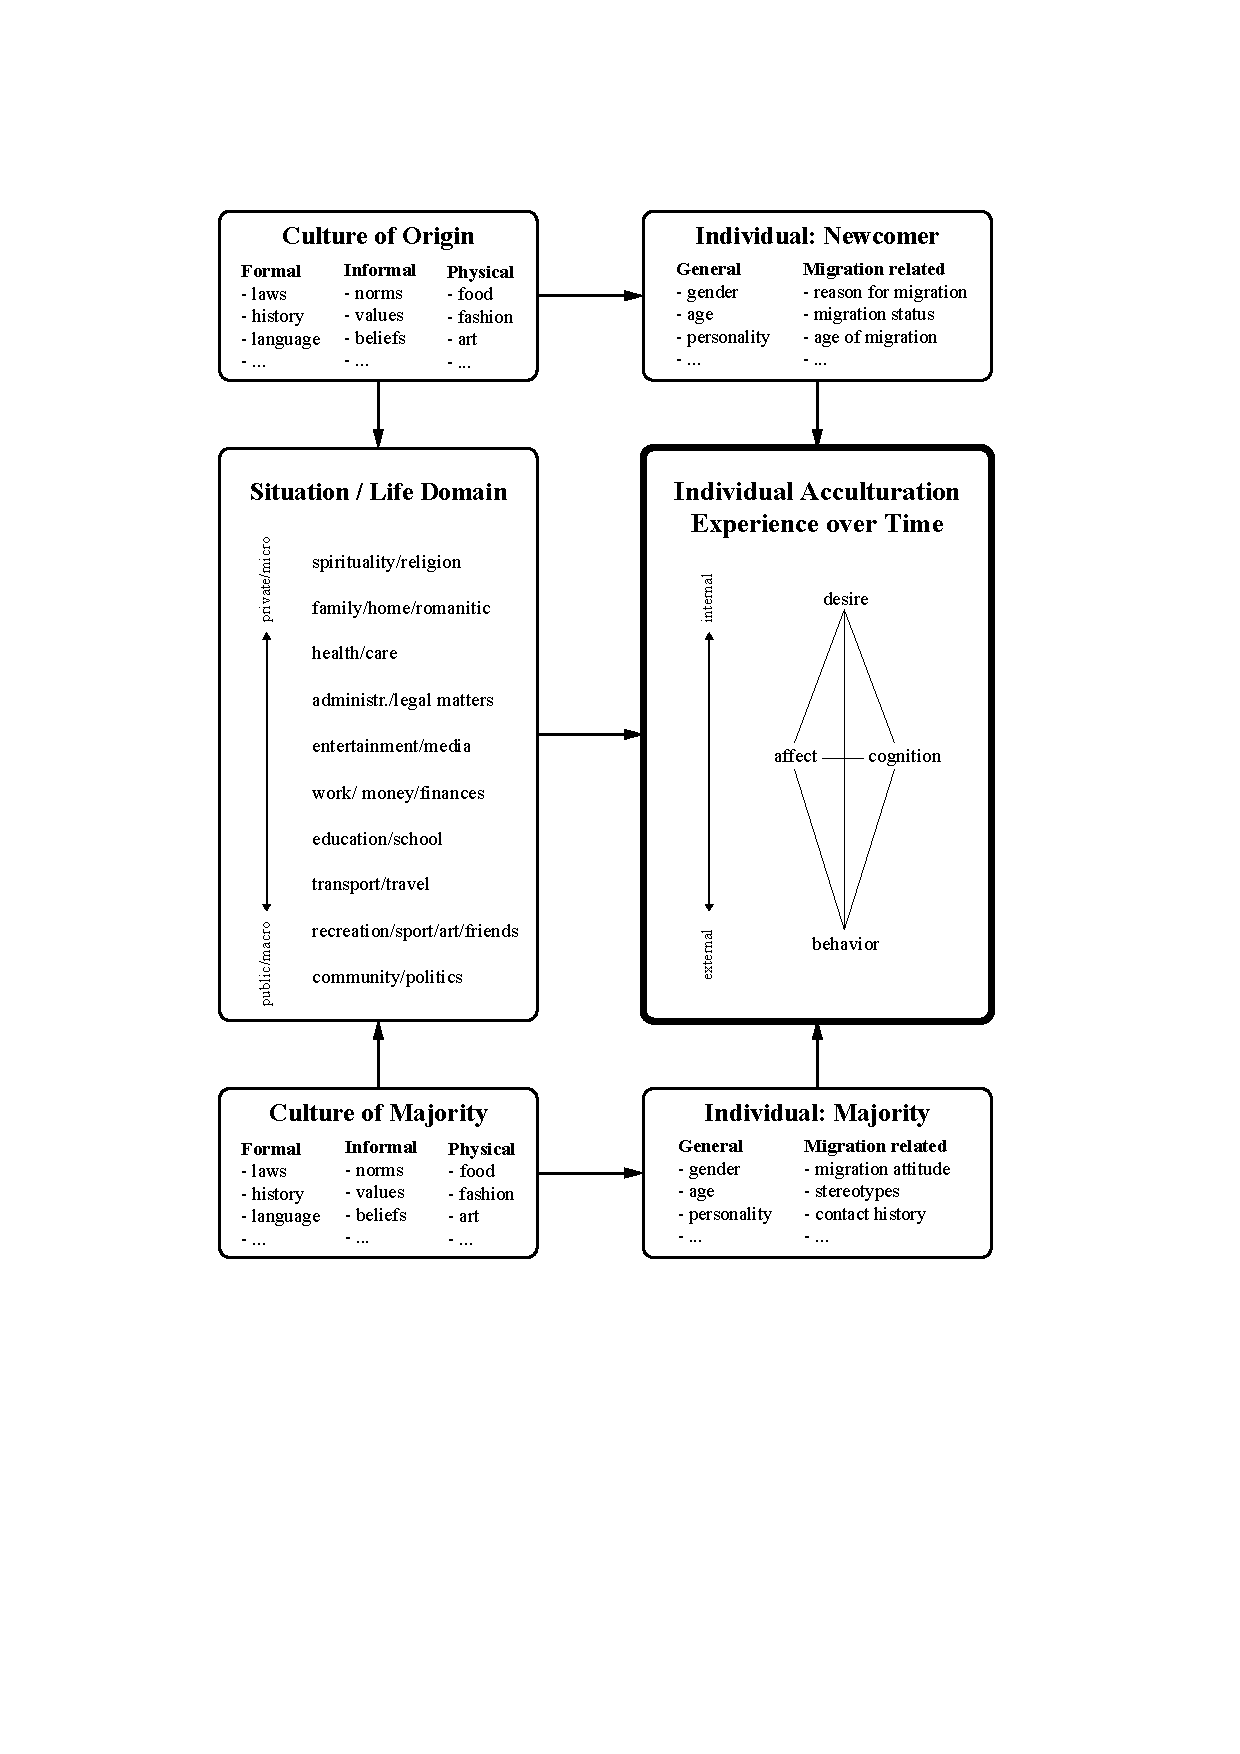
\includegraphics[width=\textwidth]{Figures/ConceptualFrameworkStatic.pdf}
\label{fig:ModelContext}
\end{figure}

\section{The present study}
The aim of our empirical efforts presented here is to put our proposed framework to the test. We have lamented that one of the challenges of a heterogeneous field is that it is difficult to assess and compare past literature. As a framework, we have suggested that the psychological elements of experiences could comprehensively structure our assessment of the literature. We will thus retrieve the past psychological literature that has proposed or used a measure of psychological acculturation and we will extract which experiential elements were considered in the research. We expect that these efforts will provide insights into the perceived importance of motives, emotions, cognitions, and behaviors for psychological acculturation. We also expect that this allows us to assess how many experience aspects are usually considered and which aspects are considered jointly. And finally, we aim to compare the understanding of psychological acculturation across different contexts and fields. 

To apply the framework, we specifically target the measurement of psychological acculturation as an operationalization of the concept within the empirical literature. We will first consider methodological literature, which aims to develop acculturation measures. Validated scales usually focus on a concept in general rather than aspects only relevant to a specific `applied' investigation. Coding psychological acculturation measures separately might also aid future considerations of measure selection because we effectively build a data base of scales that can be filtered by whether the scale includes measurements of motives, emotions, thoughts, or behaviors. Once we have considered the validated scales in particular, we will further assess the empirical literature that measures of psychological acculturation in general. Thus, in the following section we will briefly discuss how we extract key information from the literature and will then sequentially analyze the role of experience elements in the methodological and broader empirical literature of psychological psychological acculturation\footnote{It should also be noted that we consciously chose not to conduct a meta-analysis. We conduct this review exactly because we are worried about comparability across studies, a key requirement of meta-analyses \citep{Pogue1998}. In our case we, arguably, do not have a clearly defined concept and exclusions to ensure a cohesive data set would be counter productive to our efforts. Moreover, a meta-analysis is commonly understood as an analysis of analyses \citep{Glass1976}. However, since we are interested in a conceptualization (rather than a relationship, a scale metric, or population parameter) a quantitative summary in form of a meta-analysis is not well-suited to answer our research question. Also a meta-analysis of our own extracted data seems profitless because it would likely mirror a sample size weighted average.}.

\newpage
\printbibliography

\end{document}